% @Author: AnthonyKenny98
% @Date:   2020-04-08 09:56:57
% @Last Modified by:   AnthonyKenny98
% @Last Modified time: 2020-04-10 15:24:37

% @Author: AnthonyKenny98
% @Date:   2020-04-06 17:19:39
% @Last Modified by:   AnthonyKenny98
% @Last Modified time: 2020-04-06 17:29:38
\begin{figure}[H]
\begin{centering}
\includegraphics[width=0.8\linewidth]{chapters/chapter3/img/MegalongHoneyBee.png}
\mycaption{Megalong Park Honey Bee Pollinating a Weeping Cherry Blossom}{. Photographed by Emma Kenny in the Southern Highlands of New South Wales, Australia}
\end{centering}
\end{figure}

The honey bee, \textit{Apis mellifera}, has long been renowned for its tireless work ethic. However, the it is rarely given credit for its remarkable navigation and collision avoidance strategies during flight. Recent research\cite{Menzel2005} suggests that honey bees, interestingly enough, explore their workspace randomly in order to find paths from their hive to sources of pollen. Sound familiar? As such, it is quite appropriate that this functional unit, designed to work tirelessly, rapidly and efficiently to execute collision detection computations for robot motion planning, was named \textbf{HoneyBee}. \\
\bigskip

HoneyBee is a hardware unit that will eventually be incorporated into a processor, demonstrated in Figure \ref{fig:honeybee_in_processor}. In Chapter 4, the HoneyBee unit is implemented in a simple RISC-V processor and invoked using custom RISC-V instructions. For now, however, consider HoneyBee as a standalone unit that computes the grids with which an edge collides. Its resulting output can be compared to an \gls{OGM}, as explained in section \ref{subsection:EdgeCollisionFunction}.

% @Author: AnthonyKenny98
% @Date:   2020-04-08 11:15:41
% @Last Modified by:   AnthonyKenny98
% @Last Modified time: 2020-04-08 11:20:08
\begin{figure}[H]
\begin{centering}
% \includegraphics[width=\linewidth]{name}
\missingfigure[figwidth=\linewidth]{HoneyBee in a Processor}
\caption{}
\label{fig:honeybee_in_processor}
\end{centering}
\end{figure}

\subsection{HoneyBee Interface Design}
    The interface for the HoneyBee functional unit, following on from the interface specifications outlined in Section \ref{subsection:HoneyBeeTechSpechs} can be simply represented by Figure \ref{fig:honeybee_interface_simple}.

    % @Author: AnthonyKenny98
% @Date:   2020-04-08 10:23:56
% @Last Modified by:   AnthonyKenny98
% @Last Modified time: 2020-04-08 10:44:54
\begin{figure}[H]
\begin{centering}
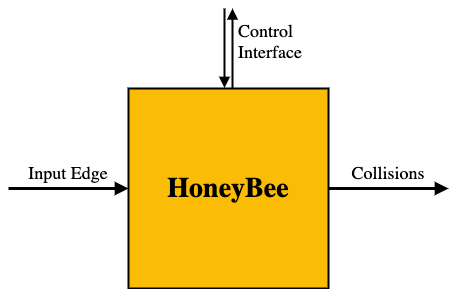
\includegraphics[width=0.6\linewidth]{chapters/chapter3/img/honeybee_interface_simple.png}
\mycaption{General Overview of HoneyBee Interface}{. The functional unit takes an edge $e$, defined by two points $p_1$ and $p_2$, as an input, and outputs a series of collisions. These collisions describe which grids an edge intersects. Its control interface allows for communication with a processors main control unit.}
\label{fig:honeybee_interface_simple}
\end{centering}
\end{figure}
    
    However, when designing hardware (the method of doing so is described in section \ref{section:honeybee_implementation}), how these inputs and outputs are implemented must be considered at the \gls{bit} level. Figure \ref{fig:honeybee_interface_detail} shows all input, output, and control ports, and their \glspl{bit-width}. 
    
    % @Author: AnthonyKenny98
% @Date:   2020-04-08 10:33:04
% @Last Modified by:   AnthonyKenny98
% @Last Modified time: 2020-04-08 11:30:28
\begin{figure}[H]
\begin{centering}
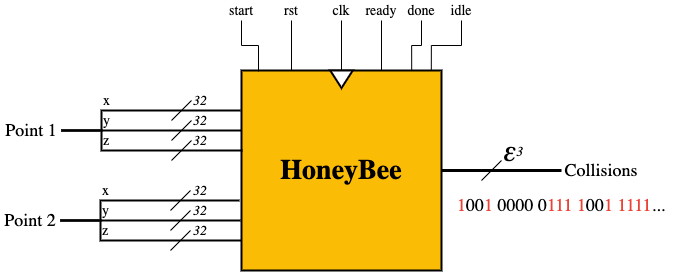
\includegraphics[width=0.8\linewidth]{chapters/chapter3/img/honeybee_interface_detail.png}
\mycaption{Port Diagram of HoneyBee Interface}{. The edge input is represented by 6 32-bit floats, following the IEEE 754 Single Precision 32-bit protocol, each float representing one of its coordinate points. The output sequence of collisions is a $e^3$-bit sequence, with each bit in the sequence representing one of the grids that was checked for intersections. It has input control signals for start and reset, and output control signals for done, idle, and ready. These control signals make up the necessary signals for a handshake protocol between HoneyBee and a processor's main controller.}
\label{fig:honeybee_interface_detail}
\end{centering}
\end{figure}

    \subsubsection{Inputs}
        The inputs to HoneyBee collectively describe a single edge. This is done with 6 32-bit floating point numbers. How floating points (non-integer numbers) are represented in binary is defined by the \gls{IEEE754}. How this is actually represented is not neccesary to understand, but is explained in Appendix \ref{section:honeybee_appendix_ieee}. The important point is that the input edge is determined by 6 32-bit coordinate points.

    \subsubsection{Output}
        HoneyBee outputs a sequence of ``collision-bits,'' with each bit in the sequence representing any collisions between the input edge with its corresponding grid. How this sequence of bits is mapped to a \gls{3D} grid-map is explained in Appendix \ref{section:honeybee_appendix_mapping}. It is important to note that in the design and implementation of HoneyBee, the length of this sequence was parameterized to be variable, corresponding to a variable value of $\epsilon$. Recall that the optimal edge collision algorithm only checked $\epsilon^3$ grids. HoneyBee, as well, only checks the grids with which the edge could possibly intersect.

        Since the number of grids being checked is parameterized, so must the number of collision-bits. This is demonstrated in Figure \ref{fig:honeybee_epsilon_grids}.
        % @Author: AnthonyKenny98
% @Date:   2020-04-08 11:48:44
% @Last Modified by:   AnthonyKenny98
% @Last Modified time: 2020-04-08 11:54:02
\begin{figure}
\begin{centering}
\begin{tabular}{c c}

    \begin{subfigure}{0.4\linewidth}
    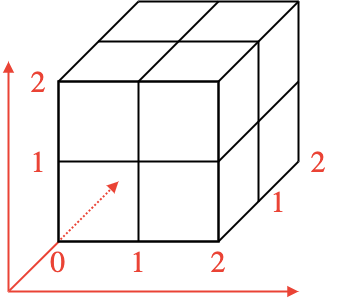
\includegraphics[width=\linewidth]{chapters/chapter3/img/honeybee_epsilon_grids_a.png}
    \caption{For $\epsilon=2$, an output collision-bit sequence of length 8 is required.}
    \end{subfigure} & 

    \begin{subfigure}{0.4\linewidth}
    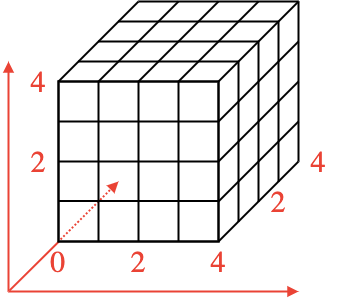
\includegraphics[width=\linewidth]{chapters/chapter3/img/honeybee_epsilon_grids_b.png}
    \caption{For $\epsilon=4$, an output collision-bit sequence of length 64 is required.}
    \end{subfigure} \\    

\end{tabular}
\mycaption{The Impact of $\epsilon$ on the Length of the Bit-Collision Sequence}{}
\label{fig:honeybee_epsilon_grids}
\end{centering}
\end{figure}

        \textbf{Note:} The output \gls{bit-width} is \textit{parameterized} not \textit{variable}. Upon synthesis (building) of HoneyBee, the output \gls{bit-width} is set at a constant value. Different syntheses may have different output \glspl{bit-width}. When the time comes to add HoneyBee to a processor, it is synthesized with a certain \gls{bit-width}.

    \subsubsection{Control Interface}
        The control interface is designed to give HoneyBee the ability to be included in a processor, and implements a commonly used ``handshake'' protocol between HoneyBee and the control unit of the processor in which it resides. Put simply, this is a method that allows the control unit to tell HoneyBee when to start executing the computation, and for HoneyBee to tell the control unit when it has finished its computation and the output value is ready. This is explained in detail in Appendix \ref{section:honeybee_appendix_handshake}. The control interface also has a clock and reset port.


\subsection{HoneyBee Implementation}
\label{section:honeybee_implementation}
    \subsubsection{Hardware Description Languages}
        Designing computers and their constituent parts has come a long way from its arduous beginnings. ``Victory'', the enigma-breaking machine designed by Alan Turing at Bletchley Park during World War II, was a large electro-mechanical computer made up of storage wheels, electromagnetic relays, and rotary switches, assembled by hand.\cite{ChoiceReviews2006} So too was ``Mark I'', the 816 cubic feet computer designed by Harvard University's Dr. Howard Aiken, which, on March 1944, computed the viability of implosion for detonating the atomic bomb.\cite{Elsabbagh2019}
        
        % @Author: AnthonyKenny98
% @Date:   2020-04-08 13:30:24
% @Last Modified by:   AnthonyKenny98
% @Last Modified time: 2020-04-08 13:54:06
\begin{figure}
\begin{centering}
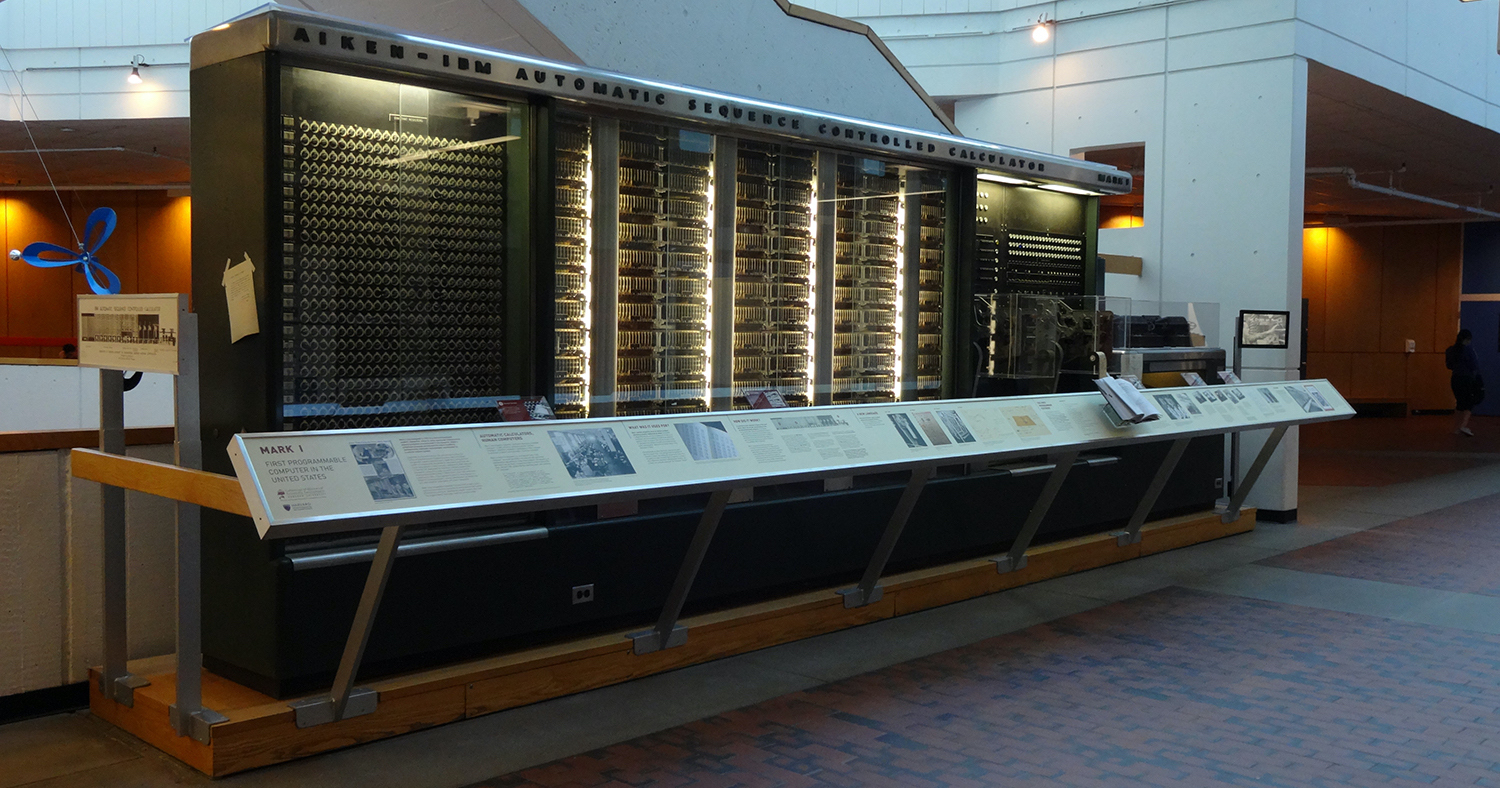
\includegraphics[width=0.7\linewidth]{chapters/chapter3/img/mark1.jpeg}
\mycaption{The Harvard Mark I Computer}{, photographed in the Harvard Science Center in April 2014 (Source: Harvard University)}
\end{centering}
\end{figure}

        Computers nowadays measure in the order of millimeters rather than meters. What's more, they are now ``built'' in software, using a \glsfirst{HDL}. \glspl{HDL} are a family of computer programming languages that are used to specify the function of electronic circuits. Tools allow for simulation of such circuits to verify design correctness and performance. Modules defined in \glspl{HDL} may then be synthesized for a type of integrated circuit called a \glsfirst{FPGA}. This \gls{FPGA}, ``programmed'' in \gls{HDL} code to behave in a certain way, can then serve the purpose of a processor or other functional processing unit. Figure \ref{fig:hdl_to_fpga} demonstrates this process.

        % @Author: AnthonyKenny98
% @Date:   2020-04-08 13:37:54
% @Last Modified by:   AnthonyKenny98
% @Last Modified time: 2020-04-08 14:00:57
\begin{figure}[H]
\begin{centering}
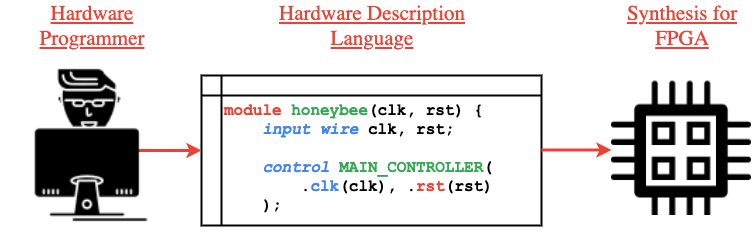
\includegraphics[width=\linewidth]{chapters/chapter3/img/hdl_to_fpga.png}
\mycaption{The Hardware Development Process}{, Defining Hardware Units in Hardware Description Languages for FPGAs.}
\end{centering}
\end{figure}

        HoneyBee was implemented eventually in an \gls{HDL} called Verilog. However, no Verilog for HoneyBee was ever explicitly written by a human. It was generated by a tool called High-Level Synthesis.

    \subsubsection{High Level Synthesis}
        \gls{HLS} is an automated hardware design process that takes design files (written in high-level languages, such as C, C++ or SystemC) specifying the algorithmic function of a piece of hardware, interprets those files, and creates digital hardware designs that execute this function. In short, it effectively translates programming languages into hardware description languages. Some key advantages of using HLS are speed and verification. It is much faster and easier to define functionality in C than it is in a \gls{HDL} such as Verilog, and thus design iterations are faster. It is also much simpler to verify one's design, as the functional units can be put through test benches written in C. \\

        The most important benefit of using \gls{HLS}, however, is the ability to use ``pragmas.'' These are directives given to the \gls{HLS} tool that tell it what optimizations to use when translating C code into an \gls{HDL}. This allows the same funtionality to be synthesized in many different ways, optimizing the synthesis for speed, area, memory, etc. As such, this hardware development process allows developers to experiment quickly with different ways to implement the same functionality. This is demonstrated graphically by Figure \ref{fig:hls_to_fpga} on Page \pageref{fig:hls_to_fpga}.

        % @Author: AnthonyKenny98
% @Date:   2020-04-08 15:17:43
% @Last Modified by:   AnthonyKenny98
% @Last Modified time: 2020-04-08 16:02:17
\begin{figure}
\begin{centering}
\begin{tabular}{c}

\begin{subfigure}{0.97\linewidth}
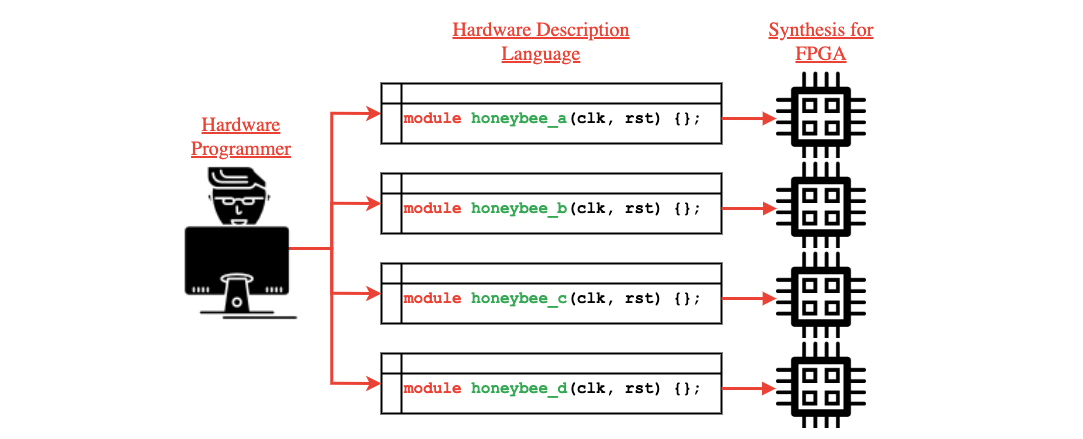
\includegraphics[width=\linewidth]{chapters/chapter3/img/hls_to_fpga_a.png}
\caption{Hardware Optimization without HLS}
\label{fig:hls_to_fpga_a}
\end{subfigure} \\

\begin{subfigure}{0.97\linewidth}
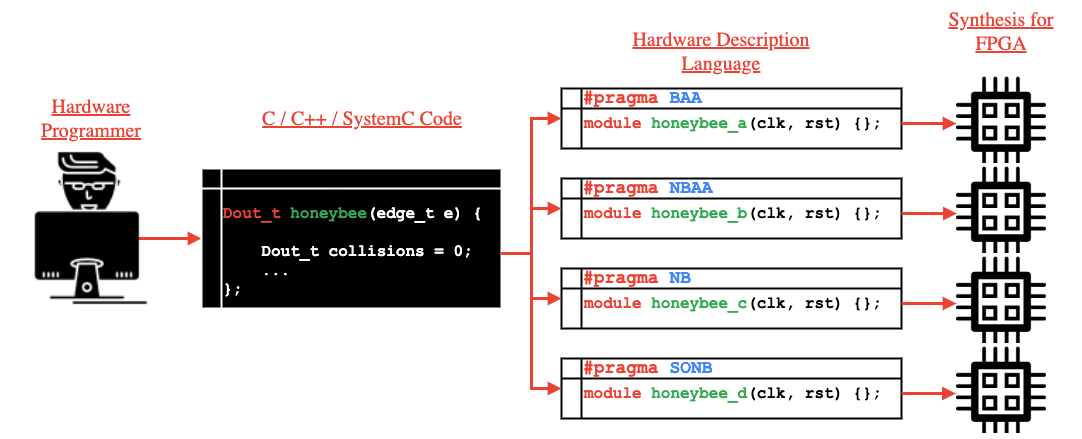
\includegraphics[width=\linewidth]{chapters/chapter3/img/hls_to_fpga_b.png}
\caption{Hardware Optimization with HLS}
\label{fig:hls_to_fpga_b}
\end{subfigure}

\end{tabular}
\mycaption{Hardware Optimization Process}{. Figure \ref{fig:hls_to_fpga_a} shows how, without using HLS, the hardware developer must write multiple different implementation of the same functionality to acheive different performance. Figure \ref{fig:hls_to_fpga_b} shows how, when using HLS, the hardware developer only must write one implementation (in a higher-level language like C), and then use ``pragmas'' to create different implementations (with different optimizations) for synthesis.}
\label{fig:hls_to_fpga}
\end{centering}
\end{figure}

    \subsubsection{HoneyBee-A Synthesis}
        With the functionality of HoneyBee implemented in C, the first optimization iteration (designated \gls{HB-A}) was synthesized. \gls{HB-A} had no pragmas, and was merely a basic hardware implementation of the defined functionality. \gls{HB-A} (and all subsequent iterations) synthesized correctly and satisfied the interface specifications (See Appendix \ref{section:honeybee_appendix_synthesis_report} for technical interface report of synthesis). Table \ref{table:HBA_results} shows the result of \gls{HB-A}'s synthesis compared with its performance and area specifications. Obviously, the synthesis is well below the area limit, but nowhere near the specifed performance metrics. This is where the beauty of High-Level Synthesis optimization comes in.

        % @Author: AnthonyKenny98
% @Date:   2020-04-08 15:34:16
% @Last Modified by:   AnthonyKenny98
% @Last Modified time: 2020-04-08 15:49:09
\begin{table}[H]
\begin{center}
\begin{tabular}{|c|c|c|}
    \hline
    \textbf{Metric}             & \textbf{Specification} & \textbf{Synthesis Result} \\
    \hline
    Latency ($\mu$seconds/edge)  &   0.9  & \textcolor{myred}{6.66} \\
    \hline
    Throughput (edges/second)  &   1,111,111 & \textcolor{myred}{150,150} \\
    \hline
    FPGA Area \glspl{LUT} & 274,080  & \textcolor{mygreen}{10,593} \\
    \hline
\end{tabular}
\mycaption{Synthesis Results for HB-A with $\epsilon = 4$}{}
\label{table:HBA_results}
\end{center}
\end{table}

\newpage
\subsection{HoneyBee Acceleration}
    This section steps through the process of using \gls{HLS} \glspl{pragma} in 2 major optimization iterations, \gls{HB-B} and \gls{HB-C} and how these iterations compared to benchmark and specified performance.

    \subsubsection{Benchmarking}
        The benchmark performance was based on a Dual-Core Intel 3.1GHz i7 processor. In an ideal world, this processor would have been chosen after a rigourous process of determining the most suitable benchmark. In reality, this processor was chosen because it was the one found in the computer running the simulations (an early 2015 MacBook Pro). Nevertheless, it serves as a suitable benchmark, demonstrating performance typical of general purpose CPUs.

        Examining latency, the benchmark was set at the average execution time for the benchmark CPU to compute 1 edge. Tests were run and averaged over 1000 trials. The average latency was 2.6 $\mu$seconds, with a standard deviation of 0.1 $\mu$seconds. This is shown, along with the performance of \gls{HB-A} in Figure \ref{fig:benchmark_1}.

        % @Author: AnthonyKenny98
% @Date:   2020-04-08 16:42:38
% @Last Modified by:   AnthonyKenny98
% @Last Modified time: 2020-04-08 17:12:56
\begin{figure}[H]
\begin{centering}
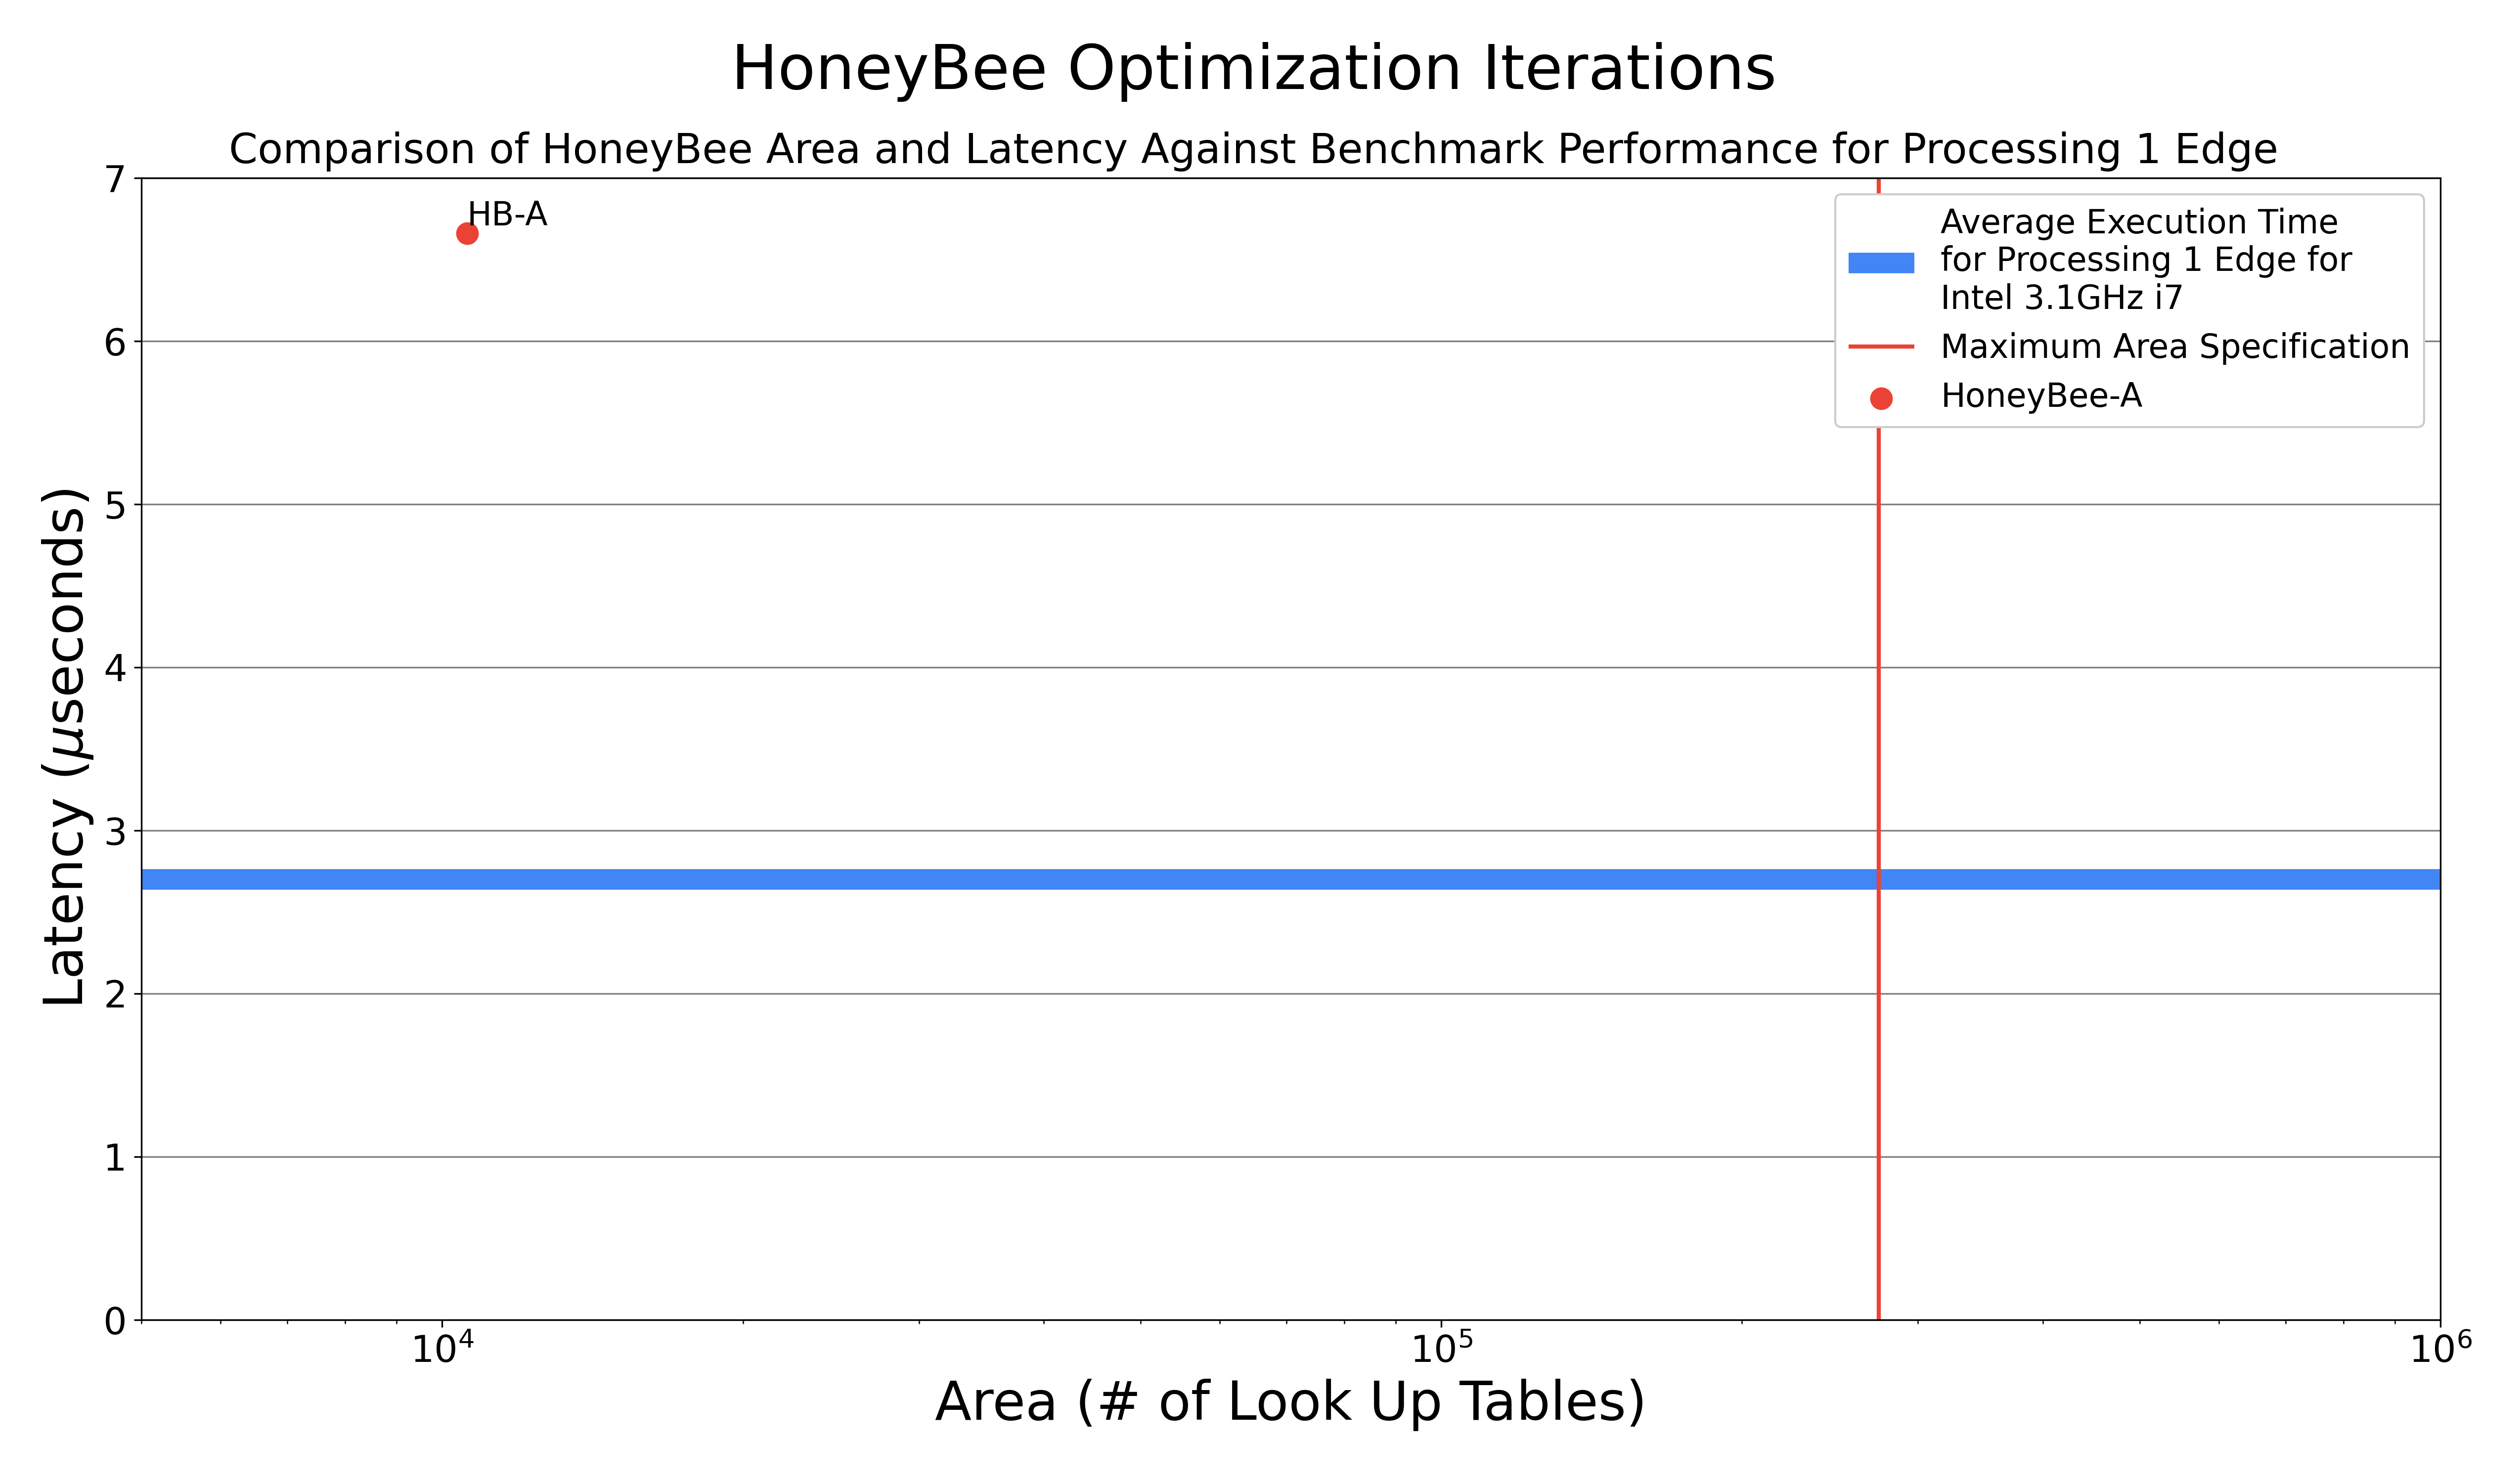
\includegraphics[width=\linewidth]{chapters/chapter3/img/benchmark_1.png}
\mycaption{HB-A Performance Against Benchmark CPU}{. Standard deviation of CPU average performance is shown by width of the line for easier interpretation.}
\label{fig:benchmark_1}
\end{centering}
\end{figure}

    \subsubsection{HoneyBee-B}
        The first step in accelerating HoneyBee was taking advantage of the inherent parrallelism available to the algorithm. Recall that the edge collision algorithm checks the $xy$-oriented planes, the $xz$-oriented planes, and finally the $yz$-oriented planes. These operations are completely independent, and can thus be performed simultaneously. Figure \ref{fig:hbb_timing} shows how the process of checking each set of planes was done sequentially in \gls{HB-A}, but are executed in parallel in \gls{HB-B}.

        % @Author: AnthonyKenny98
% @Date:   2020-04-08 18:12:53
% @Last Modified by:   AnthonyKenny98
% @Last Modified time: 2020-04-10 15:20:20
\begin{figure}[H]
\begin{centering}
\begin{tabular}{c}

\begin{subfigure}{0.97\textwidth}
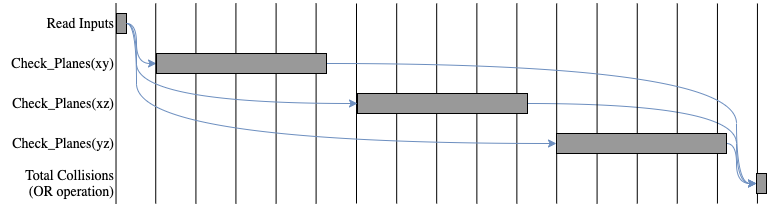
\includegraphics[width=\linewidth]{chapters/chapter3/img/timing1.png}
\caption{HoneyBee-A Timing Diagram. \texttt{Check\_Planes} executed sequentially.}
\label{fig:hbb_timing_a}
\end{subfigure} \\

\begin{subfigure}{0.97\textwidth}
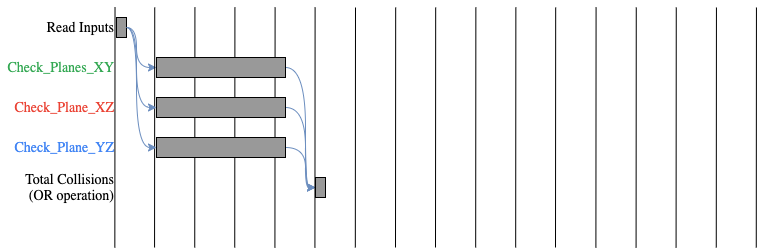
\includegraphics[width=\linewidth]{chapters/chapter3/img/timing2.png}
\caption{HoneyBee-B Timing Diagram. \texttt{Check\_Planes} executed in parallel. Different colors are to represent slightly different implementations of the same function.}
\label{fig:hbb_timing_b}
\end{subfigure} \\

\end{tabular}
\mycaption{Timing Diagrams Showing Parallelization in HoneyBee-B}{. Note, these are simlified timing diagrams for easy explanation of the concept of hardware parallelization.}
\label{fig:hbb_timing}
\end{centering}
\end{figure}

        The timing diagram does not only show the use of parallelism, it also shows how this is actually implemented in hardware. In \gls{HB-A} (Figure \ref{fig:hbb_timing_a}), there is a single module named \texttt{Check\_Plane}. Since there is only one of them, it must calculate intersections with each set of planes sequentially. On the other hand, in \gls{HB-B} (Figure \ref{fig:hbb_timing_b}), there are three separate instances of this module (\texttt{Check\_Planes\_XY}, \texttt{Check\_Planes\_XZ}, and \texttt{Check\_Planes\_YZ}), allowing HoneyBee to execute computation on all three sets of planes in parallel. 

        Moreover, notice that in \gls{HB-B}, execution time of each of these three instances is shorter than that of the single instance in \gls{HB-A}. When a single module instance is used for different purposes (in this case, checking the $xy$, $xz$, and $yz$ oriented planes), it has some variability. To control this variability, it must execute a certain amount of control logic at the beginning of the function. On the other hand, when there are seperate instances of the module, what was once variable can now be made constant. As a result, each instance can be slightly specialized and the control logic eliminated. In this case, a general \texttt{Check\_Planes} module was replaced with the three specialized \texttt{Check\_Planes\_XY}, \texttt{Check\_Planes\_XZ}, and \texttt{Check\_Planes\_YZ}. Each of these has less variability, thus less control logic, and therefore a slightly faster overall latency. Figure \ref{fig:hbb_timing} shows how theoretically, this should result in a reduction in overall latency of more than 3 times.\\

        Comparing HoneyBee-B against our benchmark, the success of this optimization can be seen. Figure \ref{fig:benchmark_2} shows the performance of multiple variants of \gls{HB-B} in yellow. These variants were the result of experimenting with slightly different \glspl{pragma}, but all fell in roughly the same area. Appendix \ref{section:honeybee_appendix_hbb_variants} lists the details of each \gls{HB-B} variant. \\
        HB-B3 showed the best performance/area relationship. It was of acceptable area and had latency marginally lower than the benchmark, but was not as fast as the defined specifications. Table \ref{table:HBB_results} shows the result of HB-B3's synthesis compared with its performance and area specifications.

        % @Author: AnthonyKenny98
% @Date:   2020-04-08 15:34:16
% @Last Modified by:   AnthonyKenny98
% @Last Modified time: 2020-04-08 19:38:23
\begin{table}[H]
\begin{center}
\begin{tabular}{|c|c|c|}
    \hline
    \textbf{Metric}             & \textbf{Specification} & \textbf{Synthesis Result} \\
    \hline
    Latency ($\mu$seconds/edge)  &   0.9  & \textcolor{myred}{2.05} \\
    \hline
    Throughput (edges/second)  &   1,111,111 & \textcolor{myred}{487,805} \\
    \hline
    FPGA Area \glspl{LUT} & 274,080  & \textcolor{mygreen}{26,524} \\
    \hline
\end{tabular}
\mycaption{Synthesis Results for HB-B3 with $\epsilon = 4$}{}
\label{table:HBB_results}
\end{center}
\end{table}

        % @Author: AnthonyKenny98
% @Date:   2020-04-08 17:54:49
% @Last Modified by:   AnthonyKenny98
% @Last Modified time: 2020-04-08 19:08:39
\begin{figure}[H]
\begin{centering}
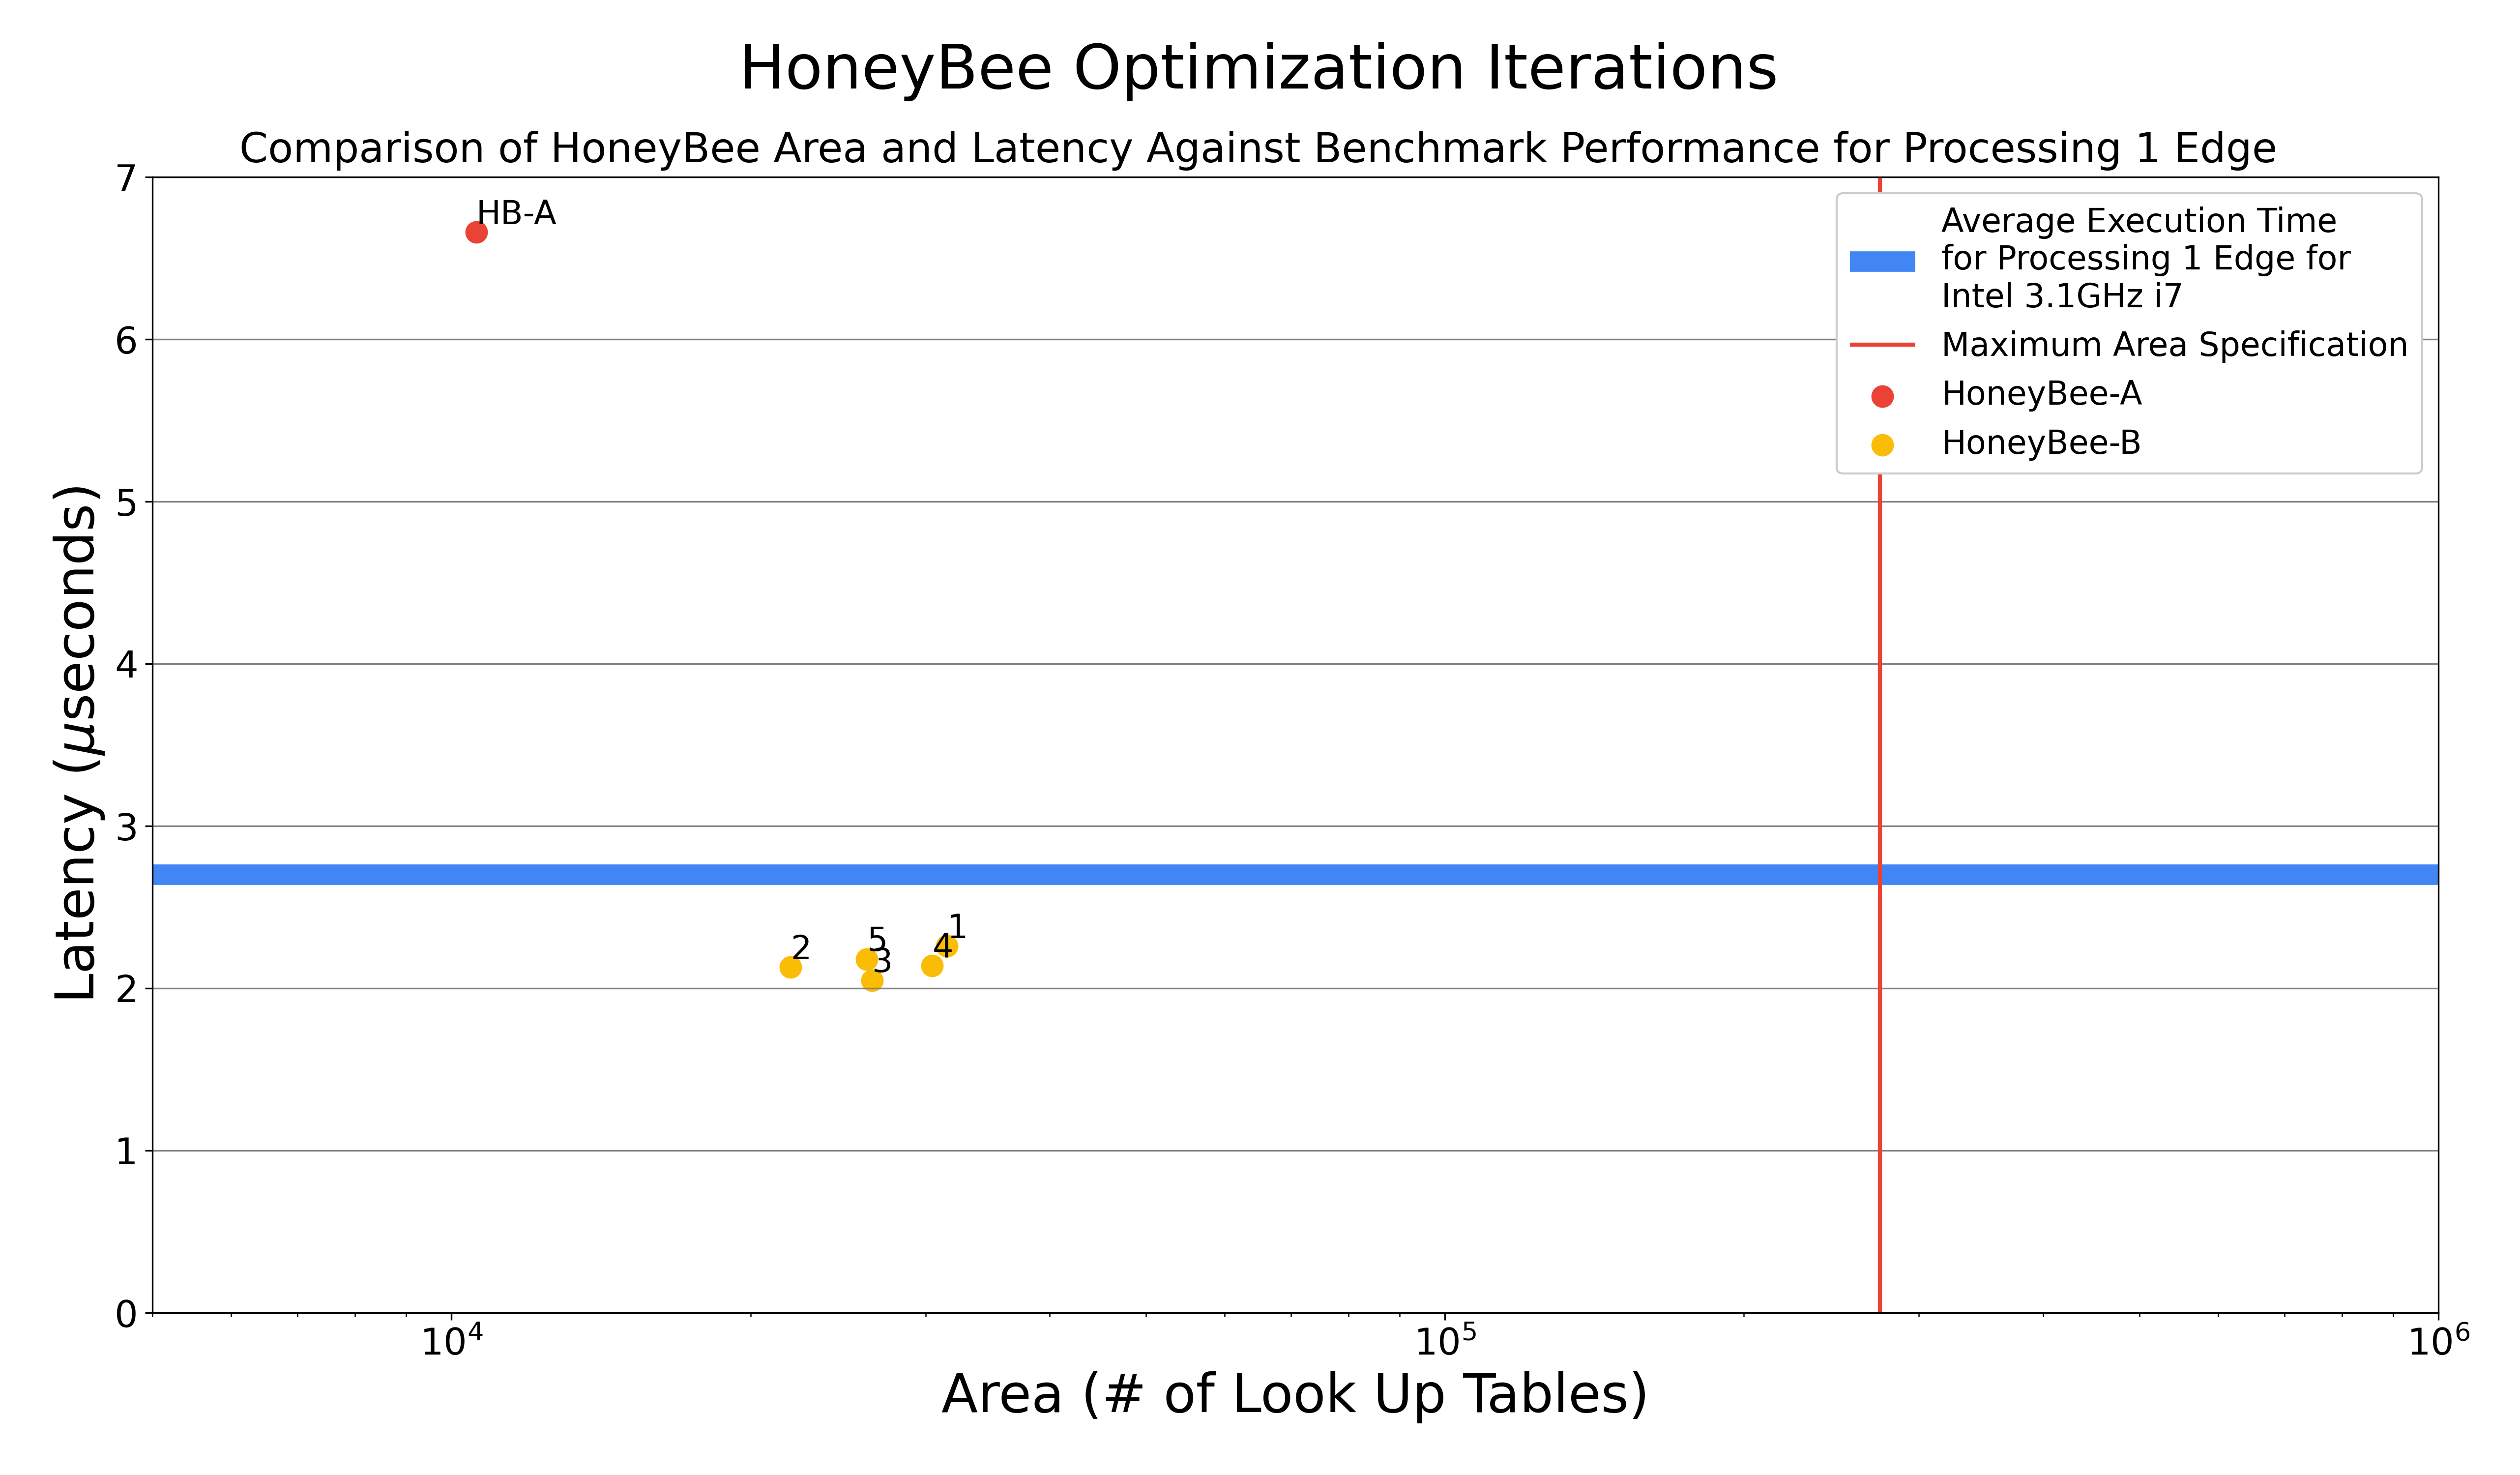
\includegraphics[width=\linewidth]{chapters/chapter3/img/benchmark_2.png}
\mycaption{HB-B Performance Against Benchmark CPU}{\\ Variants of HB-B shown in Yellow.}
\label{fig:benchmark_2}
\end{centering}
\end{figure}

    \subsubsection{HoneyBee-C}
        A similar concept was applied to optimize the computation of each set of planes. Consider synthesis of HoneyBee for $\epsilon = 4$. HoneyBee will need to compute intersections with 4 $xy$-oriented planes, 4 $xz$-oriented planes, and 4 $yz$-oriented planes. \gls{HB-B} computes each set of 4 planes simultaneously, but the computing intersections with each of the 4 planes in one orientation are also independent operations. As such, they can also be parallelized with the instantiation of more hardware modules. Figure \ref{fig:hbc_timing} shows the timing diagrams for the \texttt{Check\_Planes\_XY} module that was shown in the last set of timing diagrams.

        % @Author: AnthonyKenny98
% @Date:   2020-04-08 18:12:53
% @Last Modified by:   AnthonyKenny98
% @Last Modified time: 2020-04-08 19:21:39
\begin{figure}[H]
\begin{centering}
\begin{tabular}{c}

\begin{subfigure}{\linewidth}
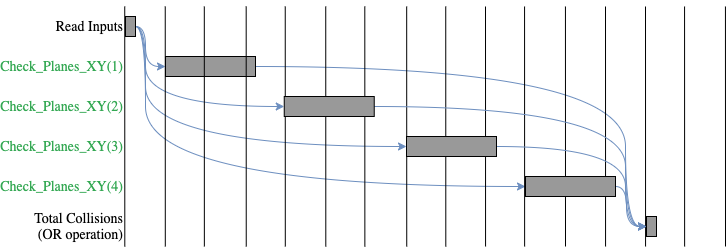
\includegraphics[width=\linewidth]{chapters/chapter3/img/timing3.png}
\caption{HoneyBee-B Timing Diagram for \texttt{Check\_Planes\_XY}. One instance of \texttt{Check\_Planes\_XY} module executed sequentially 4 times ($\epsilon=4$.}
\label{fig:hbb_timing_a}
\end{subfigure} \\

\begin{subfigure}{\linewidth}
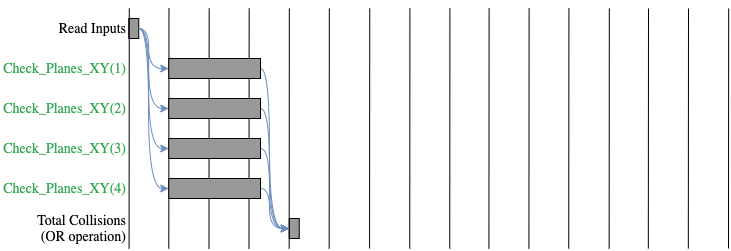
\includegraphics[width=\linewidth]{chapters/chapter3/img/timing4.png}
\caption{HoneyBee-C Timing Diagram. 4 instances of \texttt{Check\_Planes\_XY} module executing in parallel.}
\label{fig:hbb_timing_b}
\end{subfigure} \\

\end{tabular}
\mycaption{Timing Diagrams Showing Parallelization in HoneyBee-C}{. Again, these are generalizations for easy explanation of the concept of hardware parallelization. Full timing reports for each HoneyBee iteration can be found in Appendix \ref{section:honeybee_appendix_timing_reports}}
\label{fig:hbb_timing}
\end{centering}
\end{figure}

        Just focussing on the computation of the $xy$-oriented planes, Figure \ref{fig:hbc_timing} shows how \gls{HB-B} has only one instance of the module execute 4 times sequentially. \gls{HB-C}, on the other hand, implements greater parallelism by instantiating 4 module instances to execute sequentially. \gls{HB-C}, as a result, exceeded the performance benchmark and was of an acceptable area, as shown in Table \ref{table:HBC_results} and Figure \ref{fig:benchmark_3}.

        % @Author: AnthonyKenny98
% @Date:   2020-04-08 15:34:16
% @Last Modified by:   AnthonyKenny98
% @Last Modified time: 2020-04-08 19:39:39
\begin{table}[H]
\begin{center}
\begin{tabular}{|c|c|c|}
    \hline
    \textbf{Metric}             & \textbf{Specification} & \textbf{Synthesis Result} \\
    \hline
    Latency ($\mu$seconds/edge)  &   0.9  & \textcolor{mygreen}{0.53} \\
    \hline
    Throughput (edges/second)  &   1,111,111 & \textcolor{mygreen}{1,886,792} \\
    \hline
    FPGA Area \glspl{LUT} & 274,080  & \textcolor{mygreen}{185,663} \\
    \hline
\end{tabular}
\mycaption{Synthesis Results for HB-C with $\epsilon = 4$}{}
\label{table:HBC_results}
\end{center}
\end{table}

        % @Author: AnthonyKenny98
% @Date:   2020-04-08 17:54:49
% @Last Modified by:   AnthonyKenny98
% @Last Modified time: 2020-04-08 17:58:46
\begin{figure}[H]
\begin{centering}
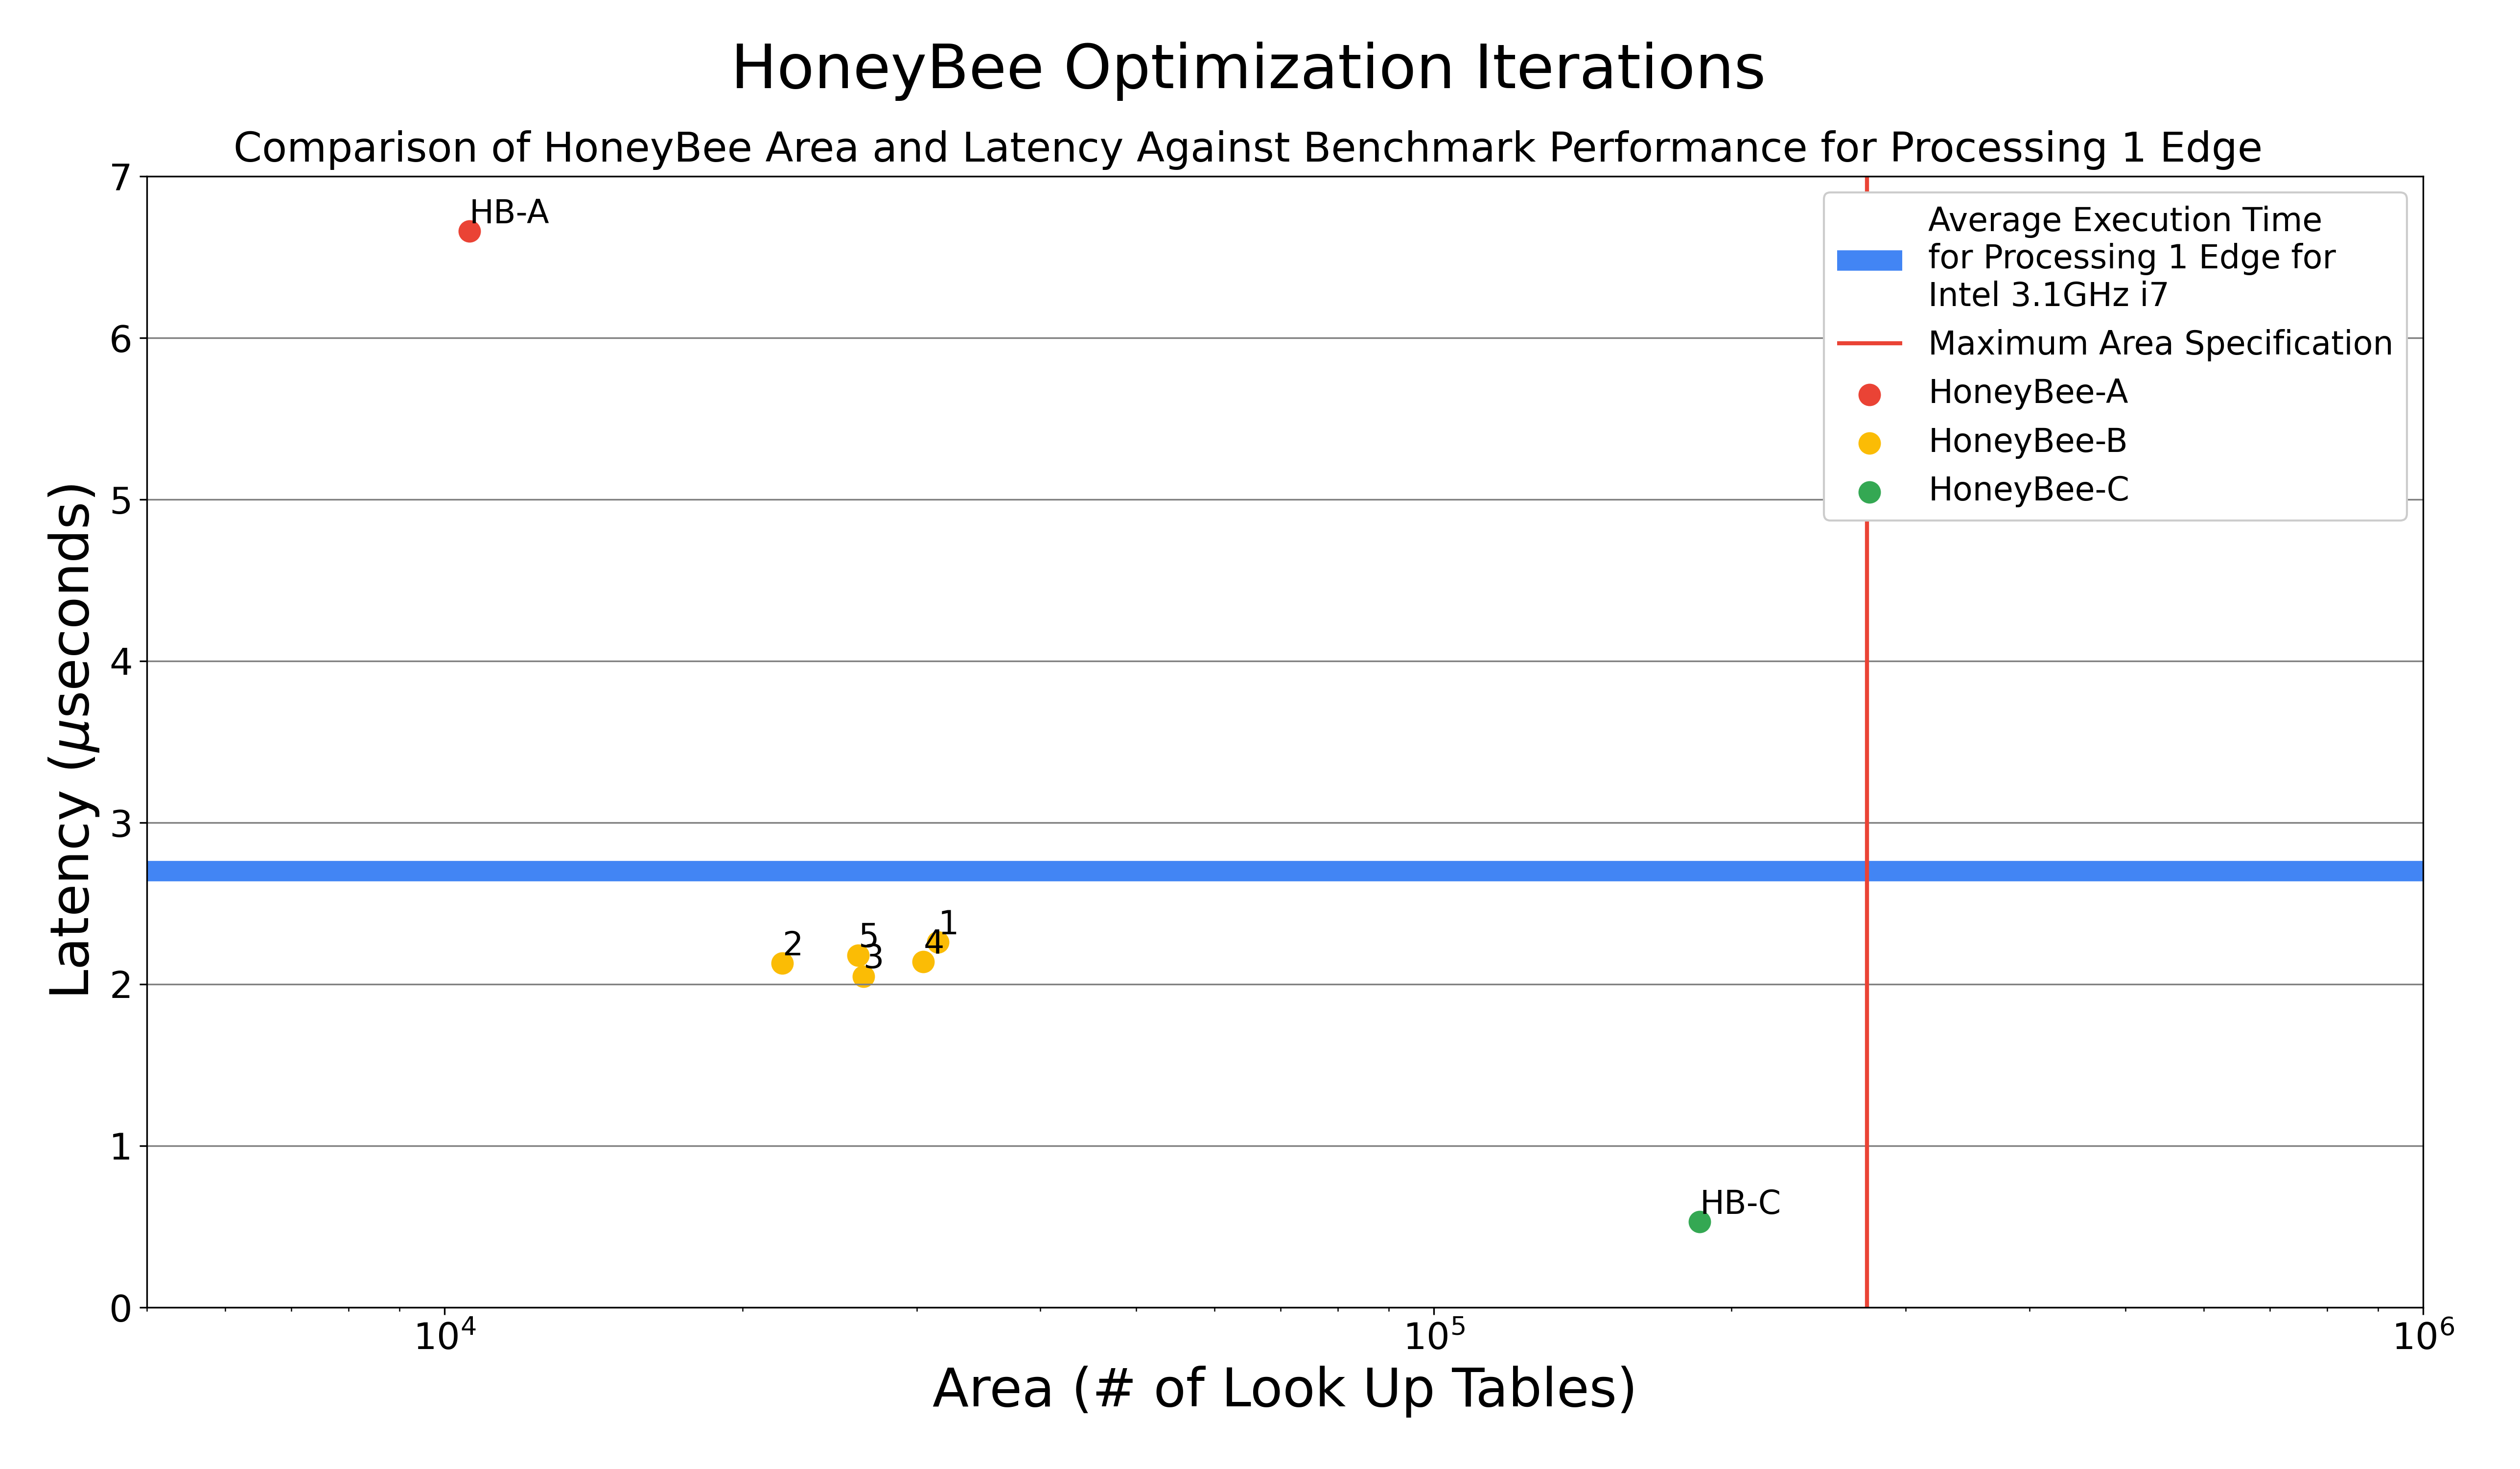
\includegraphics[width=\linewidth]{chapters/chapter3/img/benchmark_3.png}
\mycaption{}{}
\label{fig:benchmark_3}
\end{centering}
\end{figure}